\section{Physical Layer Security in reflected signals towards multiple receivers}

In real life scenarios, we deal with more than two communicating actors. We want to expand the work of chapter 3 by having it support multiple RISs in series and multiple receivers from the same transmitter. Once we have those, we can generalize it to also have receivers getting signals from multiple independent reflections of RISs.

We will first, however, make some simplifications about the actors by having $L = K$ for all of them\footnote{We want the actors to be able to communicate with each other. Since the transmitter needs to have an equal or greater number of antennas than the receiver, but the roles may later switch, it follows that the number of antennas must be equal for the calculation. Using more antennas can still be done, by not considering the values coming from them (like the original paper did as well).}. We will still consider one transmitter, with $J \ge 1$ receivers.

In this section, we consider the scenario illustrated in \cref{fig:correlation_sk2}, where a single transmitter Alice and multiple receivers exist. Frank is a direct receiver in line of sight. Bob and Charlie receive the signal from two double RIS reflections. Eve receives both the direct signal and the reflecting signal from all RISs. \footnote{It should be noted that if \textit{Eve} is in the same position as \textit{Frank} and receives just the direct signal, our particular framework would not give us physical layer security, and higher layer security would be needed. If instead \textit{Eve} has no line of sight, the message would be completely unreadable from the start, since it would receive random matrices.}

\begin{figure}[H]
  \centering
  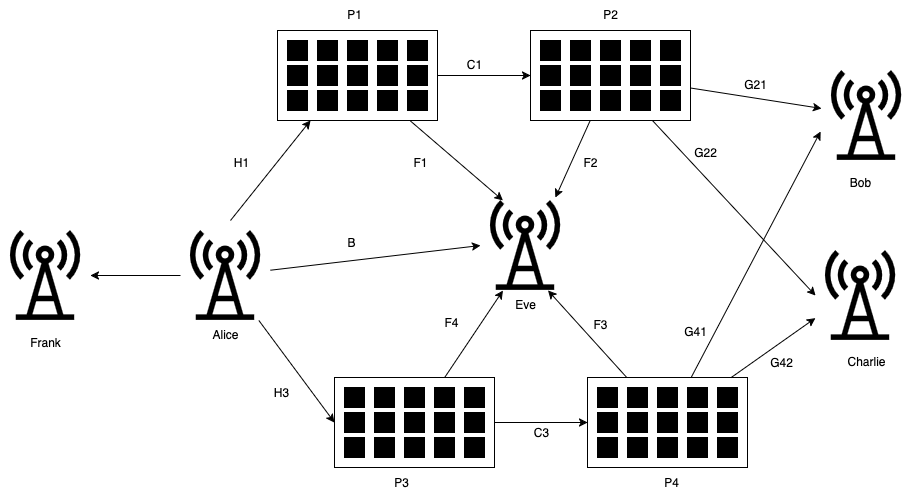
\includegraphics[width=\linewidth]{imgs/complex-situation.png}
  \caption{Complex setup for secure message transmission}
  \label{fig:correlation_sk2}
\end{figure}

More generally, we would have $M$ consecutive RIS (in series) that reflect a signal, $J$ legitimate receivers and $Q$ different paths of RIS (in parallel) to send the signal at the same time. \footnote{The paths could have a different number of RIS (for example, a path of three and another of two). The results would still hold.}

\subsection{Reflecting to multiple users}

We consider the case where the transmitter wants to send the signal to $J$ receivers without LOS. We define the link from the RIS to the receiver $j$ as $\bm{G}_j$. The condition we want to satisfy is

\begin{equation}
  \forall j \in \{1, 2, \ldots , J\} \rightarrow || \bm{G}_j\bm{PH} - [\bm{G}_j\bm{PH}]_{diag} || ^2 = 0
\end{equation}

\begin{equation}
  \forall j \in \{1, 2, \ldots , J\} \rightarrow \bm{W}_j = \sum_{i,k = 1, i \ne k}^{K} (g_{j_{k,:}} \odot h_i^T)^H (g_{j_{k,:}} \odot h_i^T)
\end{equation}

\begin{equation}
  \forall j \in \{1, 2, \ldots , J\} \rightarrow \bm{W}_j p = 0
\end{equation}

\begin{equation}
  \begin{bmatrix}
    \bm{W}_1  \\
    \bm{W}_ 2 \\
    ...       \\
    \bm{W}_J
  \end{bmatrix}
  p = 0
\end{equation}

\begin{equation}
  \begin{bmatrix}
    \bm{W}_1  \\
    \bm{W}_ 2 \\
    ...       \\
    \bm{W}_J
  \end{bmatrix}
  = \bm{W} \in \C ^ {JNxN}, \bm{W} = \bm{R \Sigma V}^H
\end{equation}

The problem we have now is that $\bm{W}$ is not a square matrix anymore, so we cannot use the last $N - (K^2 - K)$ columns of $\bm{R}$ to calculate the $\nullop$ space and $p$ with its linear combination, by using formula \eqref{null-space-hermitian}. The $\nullop$ space would have dimension $\nullop(\bm{W}) \in \C^{JN x (N - (K^2 - K))}$, but that would require a $p \in C^{JN}$ instead of $p \in C^{N}$.

We can, however, use the last $N - (K^2 - K)$ rows of $\bm{V}^H$, then apply again the hermitian transposition to get our desired solution. Remember that $N(\bm{W})$ can also be calculated using the left singular matrix, by using formula \eqref{null-space-normal}. $\bm{W}$ is not a square matrix, so $\bm{W} \ne \bm{W}^H$,

\begin{equation}
  N(\bm{W}) = \begin{bmatrix} v^H_{N - J(K^2 - K)} \\ ... \\ v^H_N \end{bmatrix} ^ H
\end{equation}

Take $\bm{U}_1 \in \C ^ {N - J(K^2 - K) \times N}$ the last $N - (K^2 - K)$ rows of $\bm{V}^H$, and
\begin{equation}
  \bm{U} = \bm{U}_1^H \in \C ^ {N x N - J(K^2 - K)}
\end{equation}

We now can apply the same method as before

\begin{equation}p = \bm{U}q\end{equation}

\begin{equation}\bm{WU} = 0\end{equation}

\begin{equation}\bm{WU}q = 0\end{equation}

\subsection{RISs in parallel}

Given the previous property, it follows that we can use $Q$ independent RISs, each one reflecting the signal to $J$ multiple receivers, and without LOS from each other. For the receiver $j \in \{1, 2, \ldots , J\}$, we have

\begin{equation}
  \sum_{m=1}^M \bm{G}_j \bm{P}_m \bm{H}_m x = (\sum_{m=1}^M \bm{G}_j \bm{P}_m \bm{H}_m) x
\end{equation}

The sum of diagonal matrices is still a diagonal matrix, so the property still holds. Remember that we only care about the indexes of the active antennas, so there is no problem in adding them together.

\subsection{RISs in series}

We consider the case where the signal is bounced between $M$ RISs with reflection matrixes $\bm{P}_1, \ldots, \bm{P}_m$ in this way:

\begin{equation}
  \text{Transmitter} \rightarrow \text{RIS 1} \rightarrow ... \rightarrow \text{RIS M} \rightarrow \text{Receiver}
\end{equation}

We call $\bm{C}_i \in \C^{N \times N}$ the channel gain between $\bm{P}_i$ and $\bm{P}_{i+1}$. We need to solve

\begin{equation}
  || \bm{GP}_1\bm{C}_1...\bm{P}_M\bm{H} - [\bm{GP}_1\bm{C}_1...\bm{P}_M\bm{H}]_{diag} || ^2 = 0
\end{equation}

We can generate $p_1, ..., p_{M-1}$ as random reflections, and calculate the last one based on the previous. An advantage we get is that eavesdroppers listening from a middle RIS will not be able to decipher the signal either.

Given $r_i \in [0, 1]$ the absorption coefficient, and $\theta_i \in [0, 2\pi]$ the phase shift, we can choose them randomly for all RIS $p_m$ vectors, but the last one.

\begin{equation}
  \forall m \in [1, M-1] : p_m[i] = \eta r_i e^{j\theta_i}
\end{equation}

Given now

\begin{equation}
  \bm{G}' = \bm{GP}_1\bm{C}_1...\bm{P}_{M-1}\bm{C}_{M-1} \in \C^{K \times N}
\end{equation}

We can consider now the problem of solving

\begin{equation}
  || \bm{G}'\bm{P}_M\bm{H} - [\bm{G}'\bm{P}_M\bm{H}]_{diag} || ^2 = 0
\end{equation}

Which can be solved as before.
\footnote{It is also possible to set up randomly the last $M-1$ RIS and calculate the first one using $\bm{G}$ and $\bm{H}'=\bm{C}_1\bm{P}_2\bm{C}_2...\bm{P}_M$. The properties still hold.}
\footnote{Estimating the channel gains $\bm{G}$ and $\bm{H}$, based on \cite{8879620}, could be more difficult, given that we do not have full control on $\bm{P}=\bm{P}_1\bm{C}_1...\bm{P}_M$ anymore. We can however estimate directly $G'$ by keeping the same random $\bm{P}_1, ..., \bm{P}_{M-1}$ in both the acknowledgment round and the message transmission round, and just modify $\bm{P}_M$ after estimating $\bm{G}'$ and $\bm{H}$ to correctly deliver the message.}

If we have multiple $\bm{G}_j$, it will be enough to calculate all the $\bm{G}'_j$ and proceed as before, allowing us to combine these properties in more complicated scenarios.

\subsection{Complex reflections}

The receiver could also get the signal from all the RISs in series, if in the right position.

For example, let's say it receives the signals $\bm{GP}_1\bm{H}_1x$ and $\bm{GP_1C_1P_2H_2}x$. To solve this system, instead of setting $\bm{P}_1$ randomly, we would need first to solve it using $\bm{G}$ and $\bm{H}_1$, then solve $\bm{P}_2$ using $\bm{G}'=\bm{GP}_1\bm{C}_1$ and $\bm{H}_2$. The sum of the two signals would still be readable for the receiver correctly.

While the calculations of $\bm{P}_1$ depend on $\bm{G}$ and $\bm{H}_1$, the signal would still be random and undecipherable for an eavesdropper receiving it.
